%%%%%%%%%%%%%%%%%%%%%%%%%%%%%%%%%%%%%%%%%%%%%%%
% ĐÂY LÀ MÃ NGUỒN CỦA FILE BÁO CÁO ĐỒ ÁN NÀY  
% Ở NGÔN NGỮ LATEX ĐỂ CHỨNG MINH BÁO CÁO NÀY  
% LÀ CỦA NHÓM TỰ SOẠN. ĐỂ ĐỌC BÁO CÁO HOÀN CHỈNH   
% THẦY VUI LÒNG XEM FILE PDF.   
%
% MẪU BÁO CÁO NÀY ĐƯỢC CUNG CẤP BỞI: OVERLEAF.COM
%%%%%%%%%%%%%%%%%%%%%%%%%%%%%%%%%%%%%%%%%%%%%%%

%%%%%%%%%%%%%%%%%%%%%%%%%%%%%%%%%%%%%%%%%
% University Assignment Title Page 
% LaTeX Template
% Version 1.0 (27/12/12)
%
% This template has been downloaded from:
% http://www.LaTeXTemplates.com
%
% Original author:
% WikiBooks (http://en.wikibooks.org/wiki/LaTeX/Title_Creation)
%
% License:
% CC BY-NC-SA 3.0 (http://creativecommons.org/licenses/by-nc-sa/3.0/)
%%%%%%%%%%%%%%%%%%%%%%%%%%%%%%%%%%%%%%%%%

\title{Báo cáo cuối kỳ Hệ thống máy tính}
%----------------------------------------------------------------------------------------
%	PACKAGES AND OTHER DOCUMENT CONFIGURATIONS
%----------------------------------------------------------------------------------------

\documentclass[12pt, final]{article}
\usepackage[a4paper, left=3cm, right=2cm, top=2cm, bottom=2cm]{geometry}
\usepackage[T5]{fontenc}
\usepackage{csquotes}
\usepackage{tabularx}
\usepackage[utf8]{inputenc}
\usepackage[vietnamese,english]{babel}
\usepackage{amsmath}
\usepackage{minted}
\usepackage{makecell}
\usepackage{titlesec}
\usepackage{unicode-math}
\usepackage{adjustbox}
\usepackage{float}
\usepackage{graphicx}
\usepackage[colorinlistoftodos]{todonotes}
\usepackage{listings}
\usepackage{longtable}
\usepackage{hyperref}

\hypersetup{
    colorlinks=true,
    linkcolor=blue,
    filecolor=magenta,      
    urlcolor=blue,
    citecolor=blue
}

\AtBeginEnvironment{minted}{%
  \renewcommand{\fcolorbox}[4][]{#4}}
  
\usepackage{etoolbox}
\patchcmd{\thebibliography}{\section*{\refname}}{}{}{}

\newcommand{\code}[1]{\texttt{#1}}

\setlength{\parindent}{0pt}
% \setlength{\parskip}{0.7em}
\renewcommand{\baselinestretch}{1.5}

\titlespacing{\section}{0pt}{0pt}{0pt}
\titlespacing{\subsection}{0pt}{0pt}{0pt}
\titlespacing{\subsubsection}{0pt}{0pt}{0pt}


\begin{document}

\begin{titlepage}

\vspace*{\fill}

\newcommand{\HRule}{\rule{\linewidth}{0.5mm}} % Defines a new command for the horizontal lines, change thickness here

\center % Center everything on the page
 
%----------------------------------------------------------------------------------------
%	HEADING SECTIONS
%----------------------------------------------------------------------------------------

\textsc{\LARGE Đại học Khoa học tự nhiên}\\[1.5cm] % Name of your university/college
\textsc{\Large Môn học: Hệ thống máy tính}\\[0.5cm] % Major heading such as course name

%----------------------------------------------------------------------------------------
%	TITLE SECTION
%----------------------------------------------------------------------------------------

\HRule \\[0.4cm]
{ \huge \bfseries BÁO CÁO ĐỒ ÁN CUỐI KỲ}\\[0.4cm] % Title of your document
\HRule \\[1.5cm]
 
%----------------------------------------------------------------------------------------
%	AUTHOR SECTION
%----------------------------------------------------------------------------------------

\begin{minipage}{0.4\textwidth}
\begin{flushleft} \large
\emph{Sinh viên:}\\
Hùng Ngọc Phát -- 19120615 \\ % Your name\\
Nguyễn Trọng Thái -- 19120652 \\
Nguyễn Hữu Nhật Tân -- 19120647
\end{flushleft}
\end{minipage}
~
\begin{minipage}{0.4\textwidth}
\begin{flushright} \large
\emph{Giảng viên:} \\
Thái Hùng Văn % Supervisor's Name
\end{flushright}
\end{minipage}\\[2cm]

% If you don't want a supervisor, uncomment the two lines below and remove the section above
%\Large \emph{Author:}\\
%John \textsc{Smith}\\[3cm] % Your name

%----------------------------------------------------------------------------------------
%	DATE SECTION
%----------------------------------------------------------------------------------------

% I don't want day because it is English
% {\large \today}\\[2cm] % Date, change the \today to a set date if you want to be precise

%----------------------------------------------------------------------------------------
%	LOGO SECTION
%----------------------------------------------------------------------------------------


\includegraphics{logo/rsz_3logo-khtn.png}\\[1cm] % Include a department/university logo - this will require the graphicx package
 
%----------------------------------------------------------------------------------------

\vspace*{\fill} % Fill the rest of the page with whitespace

\end{titlepage}

\renewcommand*\contentsname{Mục lục}
\tableofcontents

\section{Giới thiệu}
Phân công công việc:
\begin{itemize}
    \item Nguyễn Trọng Thái (19120652) và Nguyễn Hữu Nhật Tân (19120647): làm câu 1. Chi tiết hơn ghi trong mục \textbf{Câu 1}.
    \item Hùng Ngọc Phát (19120615): Làm câu 2, tổng kết báo cáo và gõ LaTeX.
\end{itemize}
Ai làm câu nào thì cũng tự soạn luôn báo cáo cho phần đó.

Mã nguồn các chương trình và nội dung báo cáo này, ngoại trừ những phần được trích dẫn, là sản phẩm trí tuệ của các thành viên nhóm.

Phần lớn kiến thức liên quan đến học phần mà không được trích dẫn đến từ tài liệu môn Hệ thống máy tính của thầy Thái Hùng Văn \cite{thaihungvan}.

Trong khi thực hiện đồ án này không thể tránh khỏi những sai sót. Nếu thầy có thắc mắc về sản phẩm của chúng em, xin thầy vui lòng liên hệ đại diện là: Hùng Ngọc Phát (19120615). Email: \code{19120615@student.hcmus.edu.vn}.

\section{Câu 1}
\subsection{Giới thiệu}
Chương trình ở câu 1 được viết bằng ngôn ngữ C++ theo chuẩn C++14 của Visual Studio. \par 
Giả sử CPU đang chạy chương trình này sử dụng kiến trúc x86 nên dữ liệu nhị phân khi đọc hoặc ghi mặc định sẽ là little endian.

\subsection{Danh sách các module}
Chương trình được chia thành các file như sau:
\begin{itemize}
    \item \code{main.cpp}: chứa hàm main và các hàm liên quan đến menu. \newline Người thực hiện: Nguyễn Trọng Thái.
    \item \code{read.h}: chứa các hàm liên quan đến việc đọc các dữ liệu từ file nhị phân theo yêu cầu đề.\newline Người thực hiện: Nguyễn Trọng Thái.
    \item \code{write.h}: chứa các hàm liên quan đến việc ghi dữ liệu xuống file nhị phân theo yêu cầu đề.
    \newline Người thực hiện: Nguyễn Hữu Nhật Tân.
    \item \code{utils.h}: các hàm tiện ích. \newline Người thực hiện: Nguyễn Hữu Nhật Tân.
\end{itemize}
Ngoài chức năng đọc/ghi chuỗi \code{UTF-16} (không thực hiện được), các chức năng còn lại theo yêu cầu đề đều hoạt động 100\% với bộ test của tụi em, bao gồm cả đọc/ghi chuỗi \code{ASCII} thay cho \code{UTF-16}.\newline
Vậy tổng thể chương trình này (Câu 1) đã hoàn thành được 80\%.

\subsection{Danh sách các hàm}
\textit{Lưu ý: cả chương trình sẽ dùng chung một biến toàn cục để thực hiện việc đọc/ghi lên file nhị phân. File này sẽ được mở/đóng từ hàm main.}
\begin{minted}[breaklines]{c}
extern FILE* f = NULL;
\end{minted}

\subsubsection{Trong module \code{main.cpp}}
\begin{itemize}
    \item \code{int main()}: Hàm main.
    \item \code{void showWriteMenu()}: để hiện menu xử lí việc ghi dữ liệu.
    \item \code{void showReadMenu()}: để hiện menu xử lí nhập dữ liệu.
\end{itemize}

\subsubsection{Trong module \code{utils.h}}
\begin{itemize}
    \item \code{static void reverseEndianess(uchar* arr, size\_t n)}: Đảo ngược một mảng có kích thước \code{n} (để chuyển đổi giữa BE với LE).
    \item \code{static char chooseEndianess()}: để yêu cầu người dùng nhập vô là nhập LE hay BE. Trả về \code{'L'} hoặc \code{'B'} tương ứng với LE và BE.\par 
    \textit{Các hàm này cần là \code{static} vì file này có thể được include nhiều lần.}
    \item Ngoài ra trong file này cũng định nghĩa kiểu viết tắt \code{uchar} thay cho \code{unsigned char} là \code{typedef unsigned char uchar;}. Tụi em sử dụng kiểu \code{unsigned char} để đảm bảo các số biểu diễn dãy byte luôn dương.
\end{itemize}


\subsubsection{Trong module \code{read.h}}
\begin{itemize}
    \item \code{void readBinary(uchar* buffer, size\_t size) }: Để đọc dữ liệu có kích thước \code{n} từ file nhị phân lưu vào \code{buffer}.
    \item \code{void docSoNguyenQuaK()}: thực hiện chức năng đọc số nguyên quá K từ file nhị phân.
    \item \code{void docSoNguyenBu2()}: thực hiện chức năng đọc số nguyên bù 2 từ file nhị phân.
    \item Các hàm khác để thực hiện các chức năng còn lại theo yêu cầu đề bài.
\end{itemize}

\subsubsection{Trong module \code{write.h}}
Tương tự như trong \code{read.h}, nhưng các hàm này dùng để ghi xuống file nhị phân các dữ liệu theo yêu cầu đề bài.

\subsection{Một số lưu ý về cơ chế hoạt động}
\begin{itemize}
    \item Để xử lí chuyển đổi giữa BE và LE, ta cần đọc các byte dữ liệu của biến cần chuyển và đưa nó vào một mảng kiểu \code{uchar[]}. Ví dụ như: biến số nguyên  \code{int a = 0xaabbccdd} (giả sử 4 byte) sẽ được lưu vào một mảng \code{uchar buffer[4] = \{0xdd, 0xcc, 0xbb, 0xaa\}} (little endian). Để chuyển nó thành big endian, ta chỉ cần đảo ngược mảng đó lại. \par 
    
    Ta cần sử dụng hàm \code{memcpy(dest\_ptr, source\_ptr, size)} của C để copy dữ liệu nhị phân từ 1 biến (nguyên, thực, ...) sang 1 mảng buffer như trên và ngược lại. Trong code thì em có dùng cú pháp \code{(uchar*)(\&a)} để ép kiểu con trỏ vùng nhớ trỏ tới \code{a} (không cần biết kiểu dữ liệu của \code{a}) sang kiểu \code{uchar*} để chuyển nó thành một dãy các phần tử, mỗi phần tử 1 byte để có thể lưu trữ cho chính xác.\cite{byteconv}\par 
    Vd: để copy dữ liệu nhị phân của 1 biến \code{double a = 2021.2022} (8 byte) thì ta có thể làm như sau:
    \begin{minted}[breaklines]{c}
    double a = 2021.2022;
    int size = 8;
    
    uchar* buffer = new uchar[size];
    memcpy(buffer, (uchar*)(&a), size);
    ...
    delete[] buffer;
    \end{minted}    
    Để làm ngược lại (chuyển dữ liệu từ byte array sang một biến nào đó), ta có thể làm như sau:
    \begin{minted}[breaklines]{c}
    long a;
    int size = 4;
    
    uchar* buffer = {0x0f, 0x0d, 0x00, 0x01};
    // Hoặc là fread(buffer, ...);
    memcpy((uchar*)(&a), buffer, size);
    ...
    delete[] buffer;
    \end{minted}  
    
    \item Khi ghi hoặc đọc một dữ liệu bất kì (kiểu int, float, ...) trong code sẽ đều được chuyển thành một byte array \code{uchar*} trước khi ghi xuống hoặc sau khi đọc lên. Nếu người dùng muốn đọc/ghi dữ liệu BE thay cho LE cũng có thể chuyển đổi một cách dễ dàng bằng phương pháp này bằng cách đảo ngược byte array đó lại.
    
    \item Trong hàm \textit{ghi} số nguyên bù 2 xuống file nhị phân, do C++ tự xử lí định dạng số nên ta chỉ cần đọc một số từ bàn phím (ko cần biết âm dương) và ghi nó xuống file là xong. Dữ liệu nhị phân trong file sẽ tự động là biểu diễn bù 2 của số nguyên đó (đã kiểm chứng qua thực nghiệm).
    \item Tuy nhiên, trong hàm \textit{đọc} số nguyên bù 2 thì do kiểu dữ liệu của biến chứa em để là \code{long long} (8 byte, để có thể chứa được mọi số nguyên có thể trong C) nên nhiều khi số nguyên của mình chỉ có 4 byte thôi, khi đọc thì 4 byte còn lại sẽ bị thiếu. Nếu nó là số âm thì mình cần gán phần bị thiếu đó bằng \code{0xfff...}, còn nó là số dương thì mình cần gán nó bằng \code{0x000...}.\par 
    Ví dụ giả sử số nguyên mà ta cần đọc là 4 byte, có dạng \code{0xffaabbcc} (số âm), nhưng biến để chứa nó là \code{long long} 8 byte. Khi đọc vào nó sẽ trở thành \code{0x00000000ffaabbcc} (số dương). Do đó ta cần xét bit dấu và chỉnh nó lại thành \code{0xffffffffffaabbcc} (số âm) mới đúng. \newline Chi tiết hơn thầy có thể xem trong chương trình.
\end{itemize}

\subsection{Chạy thử}
Ở đây em sẽ lần lượt nhập các thông tin sau:

\begin{table}[H]
\centering
\begin{tabularx}{\textwidth}{| X | X | X | X |}
\hline
\textbf{Dữ liệu} & \textbf{Giá trị (dec)} & \textbf{Kích thước} & \textbf{LE/BE} \\
\hline
Số nguyên bù 2 & -100 & 1 byte & LE \\

Số nguyên bù 2 & 2021 & 4 byte & BE \\
Số nguyên quá 100 & -70 & 4 byte & LE \\
Chuỗi ASCII & he thong may tinh & 17 kí tự & BE \\
Số thực chấm động & 192.168 & 4 byte & LE \\
\hline
\end{tabularx}
\end{table}
Nội dung file nhị phân sau khi ghi liên tiếp các thông tin trên (do gõ trên LaTex nên chèn hình hơi khó, em xin paste cho nhanh).

\begin{minted}[breaklines]{text}
00000000: 9c00 0007 e51e 0000 0000 686e 6974 2079  ..........hnit y
00000010: 616d 2067 6e6f 6874 2065 6802 2b40 43    am gnoht eh.+@C
\end{minted}

Chúng ta có thể tính (bằng tay) được các offset của các thông tin ở bảng trên lần lượt là \code{0, 1, 5, 9, 27}.
Tiếp theo ta sẽ thử chức năng đọc dữ liệu nhị phân từ các offset trên với định dạng tương ứng. Kết quả đọc được ở hình dưới đây:
\begin{figure}[H]
\centering
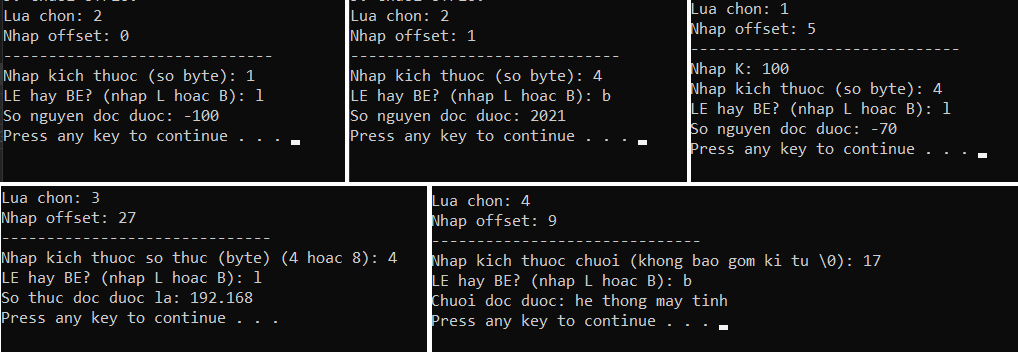
\includegraphics[width=\textwidth]{image/test.png}
\caption{Kết quả khi đọc tại các offset trên của file nhị phân đã ghi ở bước trước}
\end{figure}

Ta có thể thấy được các dữ liệu đọc được hoàn toàn khớp với các dữ liệu ta đã nhập vào.

\section{Câu 2}
\subsection{Giới thiệu}
Chương trình ở câu 2 được viết bằng hợp ngữ \code{8086}, biên dịch bởi trình hợp dịch \code{emu8086 v4.08} và được test trên \code{DOSBox 0.74-3}.\\
Chương trình không sử dụng thư viện nào khác ngoài các ngắt \code{21h, 10h} và \code{15h} của DOS cũng như BIOS.\\
Nhắc lại chức năng của chương trình:
\begin{itemize}
    \item Đọc trạng thái của 2 đèn NumLock (NL) và CapsLock (CL) [Hoàn thiện: 100\%].
    \item Nếu đèn NL và CL đều sáng, in ra ngày giờ của máy tính dưới dạng đồng hồ \textit{tự refresh sau mỗi 1 giây} [Hoàn thiện: 100\%].
    \item Nếu chỉ có đèn NL sáng, tính tổng, hiệu, tích, thương của 2 số tự nhiên $M$ và $N$ nhập từ bàn phím sao cho $0 \leq M, N < 10$ [Hoàn thiện: 100\%].
    \item Nếu chỉ có đèn CL sáng, vẽ một hình chữ nhật kích thước $M\times N$ bằng các dấu hoa thị * sao cho $M$, $N$ nhập từ bàn phím và $0 \leq M, N < 10$ [Hoàn thiện: 100\%]. 
\end{itemize}

\subsection{Sơ lược về các 8086 instruction được sử dụng trong bài này\cite{8086instruction}}
Một instruction có thể có rất nhiều lựa chọn tham số khác nhau, nhưng trong phần này em sẽ chỉ nêu các lựa chọn có sử dụng trong đồ án này mà thôi.

\subsubsection{Một số lệnh đơn giản}
Bao gồm \code{MOV, LEA, INT, Jxxx, RET, ...}

\subsubsection{\code{ADD} và \code{SUB}}

Cú pháp: \code{ADD/SUB A, B}. 

2 lệnh này nhận vào 2 tham số tổng quát là \code{A} và \code{B}, và thực hiện phép gán \code{A=A+B} hoặc \code{A=A-B}.
Trong bài này chỉ sử dụng lệnh 2 lệnh đã nêu với \code{A} là một thanh ghi 8-bit. 

\subsubsection{\code{MUL}}
Cú pháp: \code{MUL X}.

Nếu \code{X} là một byte, lệnh \code{MUL} sẽ thực hiện phép gán \code{AX=AL*X}.\\
Nếu \code{X} là một word, lệnh \code{MUL} sẽ thực hiện phép gán \code{(DX:AX)=AX*X}.

\textit{Ghi chú: kí hiệu \code{DX:AX} nghĩa là một thanh ghi 32-bit "ảo" được tổ hợp từ 2 thanh ghi 16-bit \code{DX} và \code{AX} với \code{DX} là phần high và \code{AX} là phần low.}\\
Nghĩa là giá trị chứa trong thanh ghi \code{DX:AX} là \code{DX * 10h + AX} \cite{asmbeginner}. 

\subsubsection{\code{DIV}}
Cú pháp: \code{DIV X}.

Nếu \code{X} là một byte, lệnh \code{DIV} sẽ thực hiện phép toán \code{AX/X}, sau đó lưu thương số vào \code{AL} và dư số vào \code{AH}.\\
Nếu \code{X} là một byte, lệnh \code{DIV} sẽ thực hiện phép toán \code{(DX:AX)/X}, sau đó lưu thương số vào \code{AX} và dư số vào \code{DX}.

\subsubsection{\code{PUSH} và \code{POP}}
Cú pháp: \code{PUSH/POP X} với \code{X} là thanh ghi 16-bit.

Cặp lệnh này để thao tác với ngăn xếp (stack) được implement sẵn trong VXL 8086 \cite{asmstack}. Thường được gọi một cách thủ công để backup lại dữ liệu của các thanh ghi (sau hoặc trước một quá trình tính toán nào đó) trước khi ghi đè chúng để thực hiện các công việc khác. \\
Chúng ta cũng cần lưu ý không được làm corrupt ngăn xếp này (\code{PUSH} mà không \code{POP}, hoặc \code{POP} nhiều hơn \code{PUSH}, ...) vì nó cũng được sử dụng làm callstack cho các thủ tục. Khi đó các thủ tục sau khi kết thúc sẽ bị return về sai vị trí. 

\subsection{Sơ lược về các 8086 interrupt được sử dụng trong bài này\cite{8086interrupt}}

\begin{table}[H]
\centering

\begin{tabularx}{\textwidth}{| X | X | X | X |}
\hline
\textbf{Ngắt và hàm} & \textbf{Tác dụng} & \textbf{Tham số} & \textbf{Trả về} \\
\hline
int 21h,\par AH=02h & In một kí tự ra màn hình & DL = Mã ASCII kí tự cần in & AL = DL \\
\hline
int 21h,\par AH=09h & In một chuỗi ra màn hình. Chuỗi phải kết thúc bằng dấu \code{\$} & DS:DX = địa chỉ của chuỗi & Không \\
\hline
int 21h,\par AH=0Ch & Flush input buffer và gọi một hàm đọc khác & AL = STT của hàm đọc cần gọi & Tuỳ vào hàm đọc đã gọi \\
\hline
int 21h,\par AH=4Ch & Trả quyền điều khiển về cho hệ điều hành & Không & Không \\
\hline
int 21h,\par AH=2Ah & Lấy ngày hệ thống & Không & CX = năm (1980--2099), DH = tháng, DL = ngày, AL = thứ \\
\hline
int 21h,\par AH=2Ch & Lấy giờ hệ thống & Không & CH = giờ, CL = phút, DH = giây \\
\hline
int 10h,\par AH=02h & Đặt vị trí con trỏ & DH = hàng, DL = cột, BH = trang & Không \\
\hline
int 10h,\par AH=03h & Lấy vị trí con trỏ & BH = trang & DH = hàng, DL = cột \\
\hline
int 15h,\par AH=86h & Báo BIOS đợi một khoảng thời gian & CX:AX = thời gian bằng micro giây & Không \\
\hline
\end{tabularx}

\end{table}


\subsection{Chi tiết về các hàm và thủ tục được sử dụng}
\subsubsection{Danh sách các thủ tục và chức năng}
Dưới đây là bảng tổng quát các thủ tục em đã viết thêm để có thể lập trình một cách dễ dàng hơn.

\begin{table}[H]
\centering
\begin{tabular}{|p{0.35\linewidth} | p{0.6\linewidth}|}
\hline
\textbf{Tên thủ tục}   & \textbf{Chức năng chính}  \\
\hline
main          & Hàm main                                             \\
\hline
printNumberAL & In một số có 1 hoặc 2 chữ số trong thanh ghi AL         \\
\hline
printDX       & In một chuỗi có địa chỉ trong DX                        \\
\hline
printRect     & Thực hiện chức năng in một hình chữ nhật kích thước MxN \\
\hline
calculate2Num & Thực hiện chức năng tính các phép toán trên 2 số M và N \\
\hline
showClock & Thực hiện chức năng hiển thị đồng hồ \\
\hline
\end{tabular}
\end{table}

\subsection{Hàm \texttt{main}}
Hàm main thực hiện các chức năng sau:
\begin{itemize}
    \item Nạp các biến cần thiết từ bộ nhớ vào data segment.
    \item Đọc và trích xuất các dữ liệu cần thiết từ \textit{BIOS Data Area (BDA)} \cite{bda}.
    \item Dựa vào các dữ liệu trích xuất được mà thực hiện các chức năng phù hợp theo yêu cầu đề bài.
\end{itemize}
Để đọc trạng thái các phím CapsLock (CL) và NumLock (NL), em đã đọc và trích xuất các thông tin ở BDA. Cụ thể như sau:
\begin{itemize}
    \item Dữ liệu cần thiết để đọc trạng thái các phím CL và NL gọi là \textit{Keyboard Flag Bytes}, gồm 4 byte.
    \item Chúng ta chỉ cần byte 0, nó chứa trạng thái của các phím NumLock, ScrollLock, CapsLock cũng như một số phím khác như Ctrl, Alt, ...
    \item Byte 0 của KBF nằm ở vị trí \texttt{40h:17h} trong bộ nhớ \cite{bda}, nên ta cần thêm thanh ghi đoạn \texttt{ES} để chứa giá trị \texttt{40h} (trong code hợp ngữ).
    \item Trong byte 0, chúng ta chỉ cần 2 bit là bit số 5 (trạng thái NL) và bit số 6 (trạng thái CL). 
    \begin{figure}[H]
        \centering
                \begin{minted}[breaklines]{c}
    40:17 byte Keyboard flag byte 0 (see KB FLAGS)
            
    |7|6|5|4|3|2|1|0| keyboard flag byte 0
     | | | | | | | `--- right shift key depressed
     | | | | | | `---- left shift key depressed
     | | | | | `----- CTRL key depressed
     | | | | `------ ALT key depressed
     | | | `------- scroll-lock is active
     | | `-------- num-lock is active
     | `--------- caps-lock is active
     `---------- insert is active
        \end{minted}
        \caption{Cấu trúc của ô nhớ số 17h tại offset 40h trong BDA \cite{bda}}
    \end{figure}
    \item Để đọc 2 bit này, ta gọi lệnh \texttt{SHL} (dịch trái) 3 lần và đọc các bit bị "rơi" ra qua thanh ghi cờ \code{CF}.
\end{itemize}

\subsection{Thủ tục \texttt{printDX}}
Hàm này chức năng không có gì quá đặc biệt, chỉ rút ngắn 2 dòng lệnh in chuỗi thành còn một dòng
\begin{minted}[breaklines]{asm}
lea dx, msg
mov ah, 2
int 21h
; Chuyển thành
lea dx, msg
call printDX
\end{minted}

\subsection{Thủ tục \texttt{printNumberAL}}
Vì input bị giới hạn lại là 2 số $m, n \in [0, 9] \subset \mathbf{N}$, nên kết quả nguyên dương lớn nhất có thể nhận được trong chương trình này là $m\times n = 81$. Do đó ta chỉ cần một hàm để in một số nguyên có 1 hoặc 2 chữ số ra màn hình.
Hàm này hoạt động theo nguyên lý sau:
\begin{itemize}
    \item Để chuyển giá trị của một chữ số bất kì \code{0..9} sang biểu diễn ASCII tương ứng của nó, ta cộng thêm nó với mã ASCII của chữ số \texttt{0} là \texttt{30h}.
    \item Nếu số đó chỉ có một chữ số (base case), ta cộng nó với \texttt{30h} và in giá trị nhận được ra màn hình.
    \item Nếu số đó có 2 chữ số, ta chia số đó cho 10. Khi đó ta thu được kết quả với dư số là chữ số thứ hai và thương số là chữ số thứ nhất. Sau đó, với mỗi chữ số nhận được, ta lại thực hiện tương tự như base case.
\end{itemize}

\subsection{Thủ tục \texttt{printRect}}
Hàm này để thực hiện chức năng vẽ hình chữ nhật có kích thước $M\times N$ với $M, N$ nguyên dương, có một chữ số, được nhập từ bàn phím.

Cách thực hiện khá đơn giản, ta chỉ cần sử dụng 2 vòng lặp lồng nhau như sau (mã giả C, đã tối ưu để dễ chuyển qua hợp ngữ hơn):
\begin{minted}[breaklines]{c}
int M, N; // 2 kích thước của hcn nhập từ bàn phím
scanf("%d %d", &M, &N);
int m = M, n = N; // 2 biến chạy
while (m > 0) {
    printf("\r\n");
    n = N;
    do {
        printf("*");
        n--;
    } while (n > 0);
    m--;
}
\end{minted}
Khi chuyển qua hợp ngữ, ở các vị trí của từ khoá \texttt{while} ta chỉ cần thay bằng các cặp lệnh \texttt{cmp} và \texttt{jxx}. Cụ thể hơn thầy có thể xem source code của chương trình.

\subsection{Thủ tục \texttt{calculate2Num}}
Hàm này để thực hiện chức năng tính các giá trị tổng, hiệu, tích, thương của 2 số tự nhiên $m, n$ thoả điều kiện trong yêu cầu đề bài.
\begin{itemize}
    \item Với tổng $m+n$ và tích $m\times n$, ta lần lượt sử dụng các instruction \texttt{add} và \texttt{mul}. 2 công việc này khá đơn giản nên em sẽ không giải thích thêm nhiều.
    \item Với hiệu $m-n$ thì khó hơn một tí, đó là ta phải xét trường hợp $m<n$, khi đó hiệu là một số âm. Hàm \texttt{printNumberAL} mà em đã viết không handle được số âm nên ta "lách luật" một chút, đó là tính và in giá trị $n-m > 0$ ra màn hình, sau đó in thêm dấu trừ ở đằng trước là được. Còn trong trường hợp $m>n$ thì hiệu $m-n>0$ nên ta làm tương tự như với tổng.
    \item Với phép chia thì khá là phức tạp, vì kết quả không phải lúc nào cũng nguyên. Để biểu diễn kết quả của $m\div n$, em sẽ sử dụng kết quả của phép chia Euclide \cite{euclide}:
    \begin{align*}
        m &= nq + r \\
        \Leftrightarrow \frac{m}{n} &= q + \frac{r}{n}
    \end{align*}
    Ví dụ, khi $m=9, n=2$ thì $q=4, r=1$ nên kết quả được hiển thị ra màn hình sẽ là \texttt{4+1/2}. Còn khi $r=0$ thì ta không cần hiển thị phần từ dấu \texttt{+} trở đi nữa.
\end{itemize}

\subsection{Thủ tục \code{showClock}}
Hàm này để hiển thị một đồng hồ đơn giản bao gồm thứ, ngày, tháng, năm và giờ, phút, giây lấy từ hệ thống (sử dụng các hàm \code{2Ah} và \code{2Ch} của ngắt \code{21h}).

Thứ tự thực hiện các chức năng của hàm này như sau:
\begin{itemize}
    \item Hiện ra các thông báo cần thiết như \code{Hom nay la ...}, \code{Bay gio la ...}.
    \item Ghi lại vị trí của của con trỏ mà tại đó cần hiển thị ngày và giờ. Vị trí để hiển thị ngày là ngay sau câu thông báo \code{Hom nay la}, còn vị trí hiển thị giờ là ngay sau câu thông báo \code{Bay gio la}.
    \item Thực hiện một vòng lặp vô hạn đến khi người dùng nhấn giữ nút \code{CTRL} thì thôi:
    \begin{itemize}
        \item Di chuyển con trỏ đến vị trí cần hiển thị ngày. Đọc ngày của hệ thống và hiển thị nó ra màn hình. Ngày được in có định dạng tương tự như: \\
        \code{Thu 3, 05/05/2021}
        \item Di chuyển con trỏ đến vị trí cần hiển thị giờ. Đọc giờ của hệ thống và hiển thị nó ra màn hình. Giờ được in có định dạng tương tự như: \\
        \code{15:23:01}.
        \item Yêu cầu BIOS nằm chờ 1 giây. Để làm được như vậy, ta cần gán số 1 triệu (micro giây) vào thanh ghi tổ hợp \code{CX:AX} và gọi hàm số \code{86h} của ngắt \code{15h}.\\ 1 triệu ở hệ 16 là \code{000f 4240h}, vậy \code{CX = 0fh} và \code{AX = 4240h}.
        \item Đọc dữ liệu của byte \code{40h:17h} từ \code{BIOS Data Area} tương tự như đầu chương trình để đọc trạng thái phím CTRL. Thực hiện shift right 3 lần để lấy bit biểu diễn trạng thái phím CTRL.
        \item Nếu bit đó là 1, thoát khỏi vòng lặp. Nếu không, tiếp tục lặp.
    \end{itemize}
    \item Kết quả ta thu được có định dạng tương tự như sau:
    \begin{minted}[breaklines]{text}
    Hom nay la Thu 3, 05/05/2021
    Bay gio la 15:23:01
    \end{minted}
    
\end{itemize}

\subsection{Biên dịch và chạy}
Chương trình được dịch bằng trình hợp dịch \code{emu8086 v4.08} và chạy thử trong trình giả lập \code{DOSBox 0.74-3}.

Các chức năng đều hoạt động ổn định, không phát sinh bất cứ lỗi nào nghiêm trọng.

Đôi khi (có lẽ do trình giả lập) mà phím NumLock khi không nhấn vẫn bị xem là có nhấn hoặc ngược lại, phải thoát trình giả lập rồi mở lại mới khắc phục được.

\textbf{Lưu ý:} để tránh phát sinh lỗi hiển thị do con trỏ màn hình hay nhảy đi lung tung, thầy vui lòng luôn luôn chạy lệnh xoá màn hình \code{cls} trên shell của DOSBox trước khi chạy chương trình để tránh màn hình bị cuộn làm sai lệnh các toạ độ đã lưu.

Một số hình ảnh trong quá trình chạy thử \textit{(trang sau)}:

\begin{figure}[H]
\centering
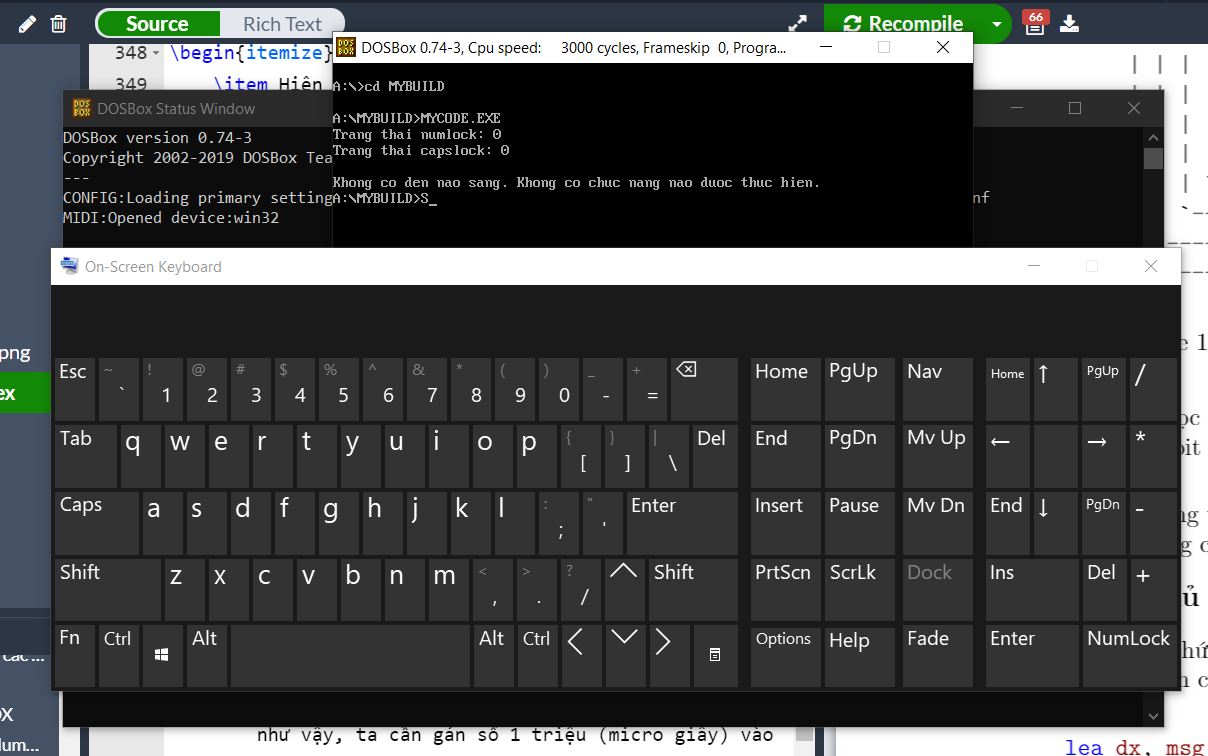
\includegraphics[width=\textwidth]{image/no-key.png}
\caption{Khi không có phím nào được nhấn}
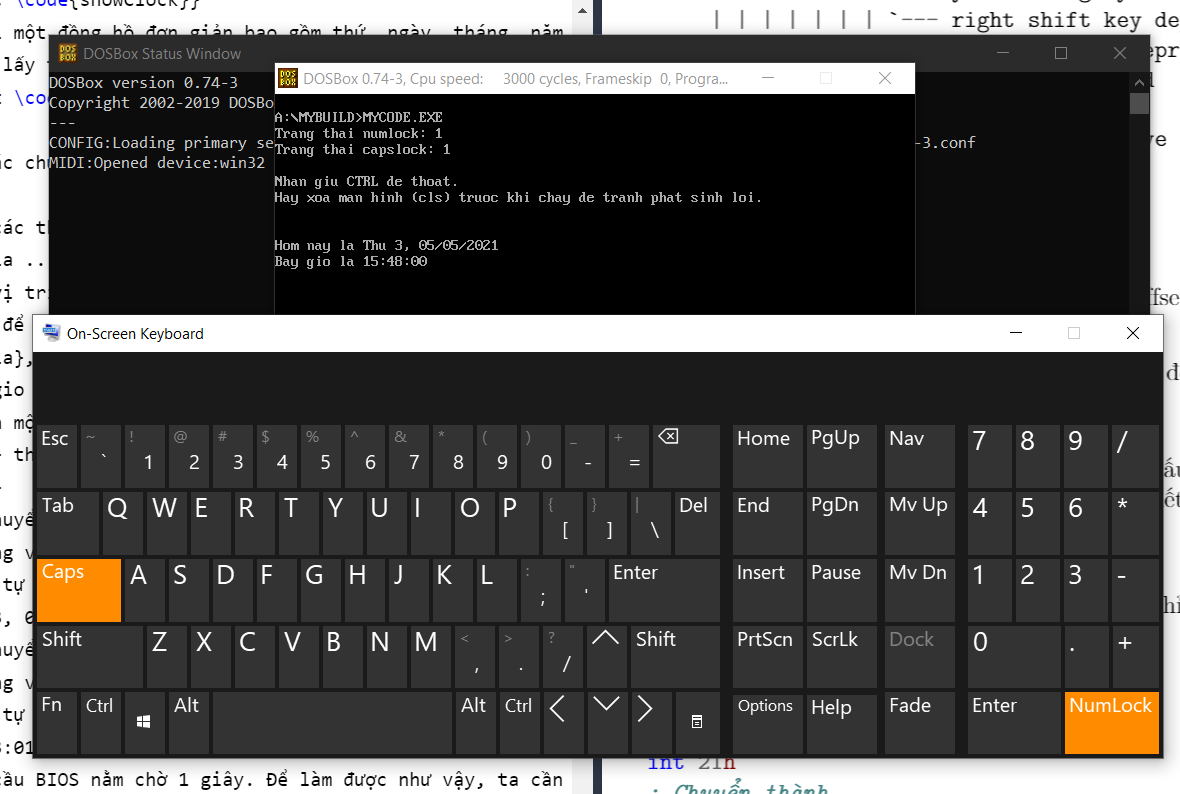
\includegraphics[width=\textwidth]{image/caps-num.png}
\caption{Khi cả 2 phím được nhấn}
\end{figure}

\begin{figure}[H]
\centering
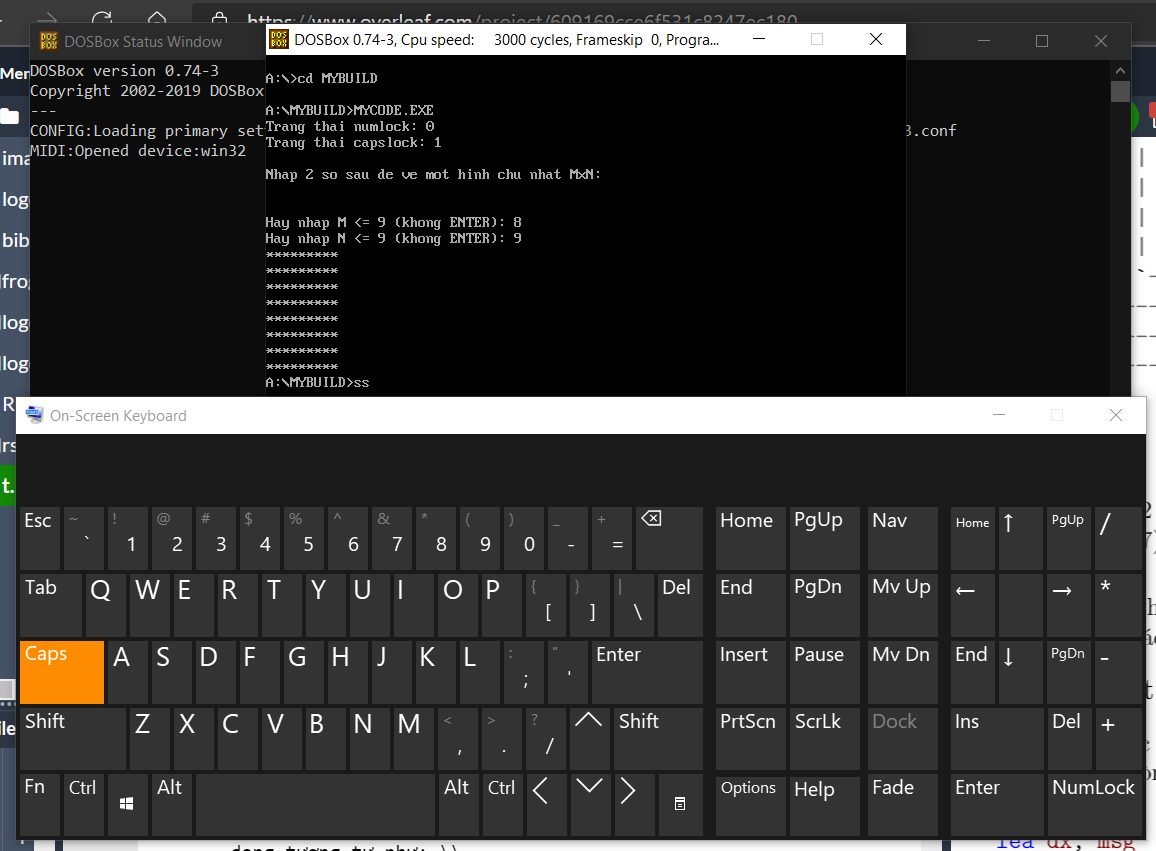
\includegraphics[width=\textwidth]{image/capslock-only.png}
\caption{Khi chỉ có CapsLock được nhấn}
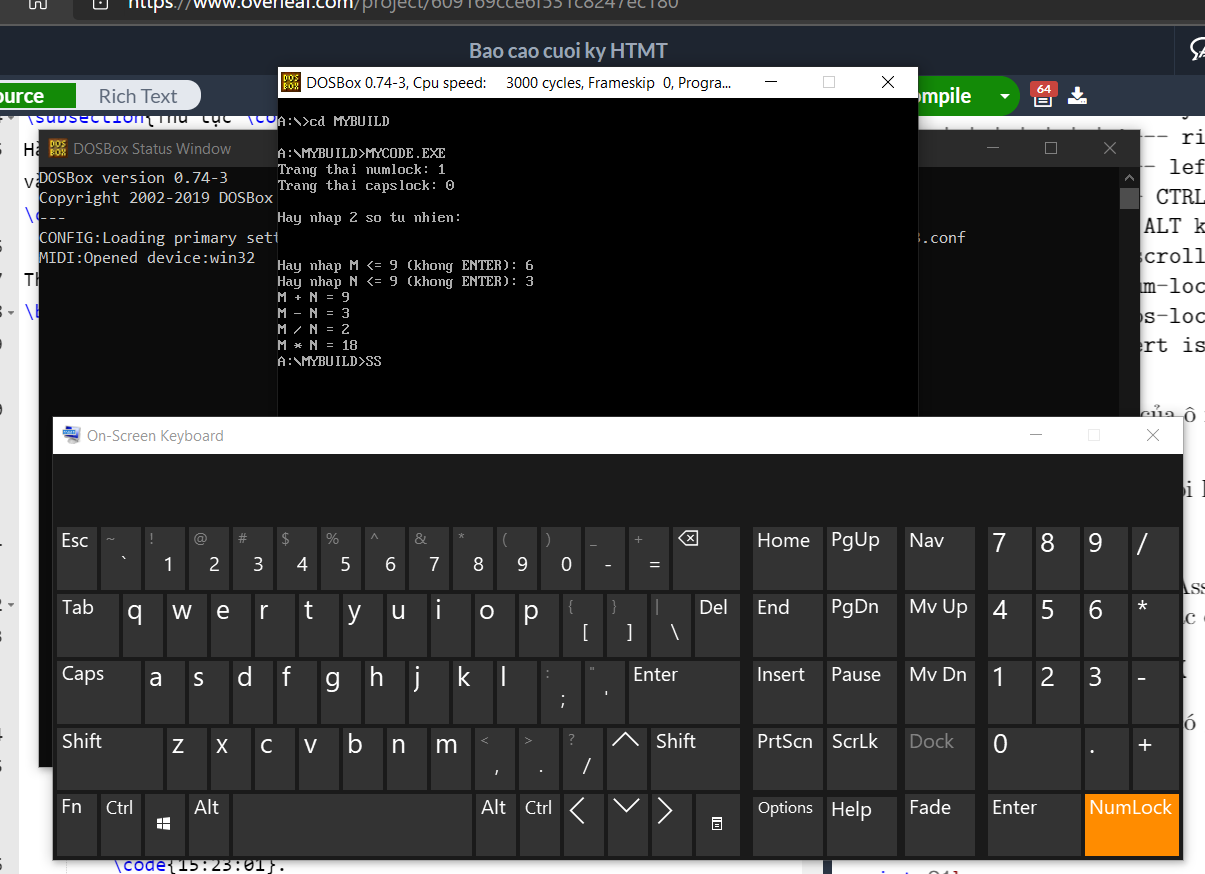
\includegraphics[width=\textwidth]{image/numlock-only.png}
\caption{Khi chỉ có NumLock được nhấn}
\end{figure}

\section{Tài liệu tham khảo}
\nocite{*}
\bibliographystyle{IEEEtran}
\bibliography{bib}

\center\textbf{Hết}

%%%%%%%%%%%%%%%%%%%%%%%%%%%%%%%%%%%%%%%%%%%%%%%%%%%%
% Comments can be added to the margins of the document using the \todo{Here's a comment in the margin!} todo command, as shown in the example on the right. You can also add inline comments too:

% \todo[inline, color=green!40]{This is an inline comment.}



% \subsection{Tables and Figures}

% Use the table and tabular commands for basic tables --- see Table~\ref{tab:widgets}, for example. You can upload a figure (JPEG, PNG or PDF) using the files menu. To include it in your document, use the includegraphics command as in the code for Figure~\ref{fig:frog} below.

% % % Commands to include a figure:
% % \begin{figure}
% % \centering
% % 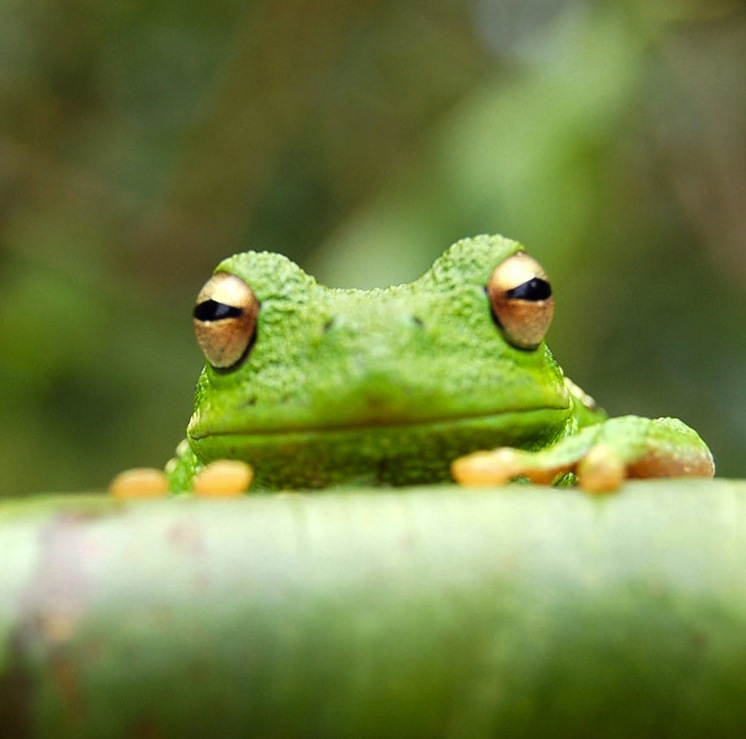
\includegraphics[width=0.5\textwidth]{frog.jpg}
% % \caption{\label{fig:frog}This is a figure caption.}
% % \end{figure}

% % \begin{table}
% % \centering
% % \begin{tabular}{l|r}
% % Item & Quantity \\\hline
% % Widgets & 42 \\
% % Gadgets & 13
% % \end{tabular}
% % \caption{\label{tab:widgets}An example table.}
% % \end{table}

% \subsection{Mathematics}

% \LaTeX{} is great at typesetting mathematics. Let $X_1, X_2, \ldots, X_n$ be a sequence of independent and identically distributed random variables with $\text{E}[X_i] = \mu$ and $\text{Var}[X_i] = \sigma^2 < \infty$, and let
% $$S_n = \frac{X_1 + X_2 + \cdots + X_n}{n}
%       = \frac{1}{n}\sum_{i}^{n} X_i$$
% denote their mean. Then as $n$ approaches infinity, the random variables $\sqrt{n}(S_n - \mu)$ converge in distribution to a normal $\mathcal{N}(0, \sigma^2)$.

% \subsection{Lists}

% You can make lists with automatic numbering \dots

% \begin{enumerate}
% \item Like this,
% \item and like this.
% \end{enumerate}
% \dots or bullet points \dots
% \begin{itemize}
% \item Like this,
% \item and like this.
% \end{itemize}

% We hope you find write\LaTeX\ useful, and please let us know if you have any feedback using the help menu above.

\end{document}